\chapter{Digital Evidence Examination and Analysis}

\section{Filesystem Structure and Organization}
Digital evidence analysis requires meticulous examination of the filesystem structure to identify potential evidence locations and understand the organizational logic employed by the user. This process involves analyzing partition layouts, file distribution patterns, and directory hierarchies to construct a comprehensive map of the digital environment. Such analysis often reveals critical insights into user behavior, including attempts to conceal information through strategic placement or mislabeling.

\subsection{Partition Analysis and Storage Architecture}
Initial examination of the imaged drive revealed a dual-partition structure with significant forensic implications. As shown in Figure 6.1, the storage media contained:

\begin{itemize}
    \item An unallocated partition labeled 'vol1 (Unallocated: 0-63)' containing potential remnants of deleted data
    \item A primary Win95 FAT32 (LBA) partition labeled 'vol2 (Win95 FAT32: 0x0c: 63-3915584)' housing the main filesystem
\end{itemize}

\begin{figure}[h]
    \centering
    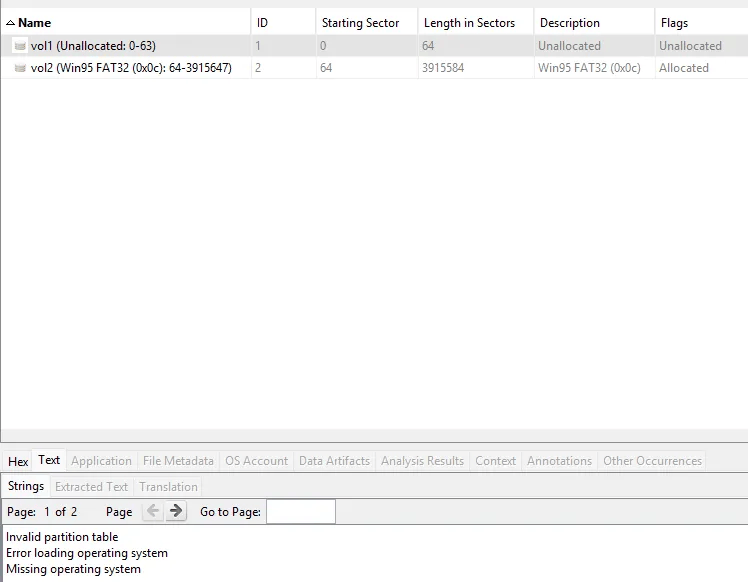
\includegraphics[width=0.8\textwidth]{images/Evidence Examination/Image1.png}
    \caption{Autopsy Partition Analysis View showing the dual-partition structure}
    \label{fig:partition_structure}
\end{figure}

The presence of the FAT32 filesystem is particularly noteworthy within the context of a contemporary investigation. While NTFS has been the standard Windows filesystem since Windows XP, FAT32 remains common on removable media and devices requiring cross-platform compatibility. In this case, the older filesystem architecture suggests either a deliberate configuration choice or the use of an older system—both possibilities having investigative significance. The FAT32 filesystem also lacks certain security features present in NTFS, such as robust permission structures and encryption capabilities, which may indicate a preference for simplicity or portability.

Examination of the partition details revealed notable findings. The unallocated space (vol1) consists of only 64 sectors, while the primary FAT32 partition (vol2) comprises 3,915,584 sectors, indicating a substantial storage volume. As visible in Figure 6.1, the partitions are properly flagged as "Unallocated" and "Allocated" respectively, with clear starting sector information that helps establish the physical layout of the data.

\subsection{File Type Distribution Analysis}
Comprehensive categorization of file types within the image reveals significant patterns in data storage and potential areas for focused investigation. Figure 6.2 illustrates the distribution of file types across the storage volume:

\begin{figure}[h]
    \centering
    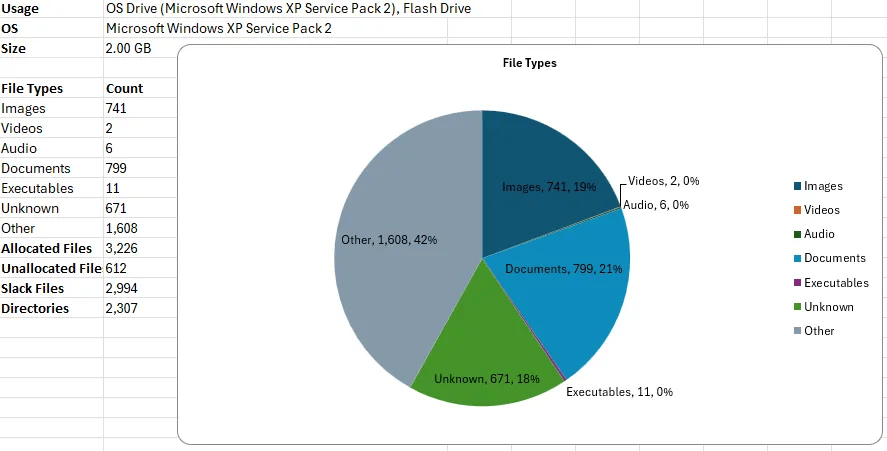
\includegraphics[width=0.8\textwidth]{images/Evidence Examination/Image2.png}
    \caption{File Type Distribution Analysis showing proportions of various file categories}
    \label{fig:file_types}
\end{figure}

This analysis revealed several notable characteristics:

\begin{itemize}
    \item A disproportionately large segment categorized as "Other" (42\%), suggesting potential use of non-standard file formats or obfuscation techniques
    \item Significant concentration of document files (21\%), indicating substantial text-based content creation or storage
    \item Images constituting a considerable portion (19\%) of the total files, warranting examination for steganographic content
    \item An "Unknown" category comprising 18\% of files, raising concerns about deliberate file type obfuscation
    \item Limited presence of executable files, audio, and video content
\end{itemize}

Additional metadata visible in Figure 6.2 reveals that the system is running Microsoft Windows XP Service Pack 2 with a total size of 2.00 GB. The drive appears to have been classified as both an OS Drive and a Flash Drive, suggesting a portable storage medium with an operating system installation. The file count breakdown shows 741 images, 2 videos, 6 audio files, 799 documents, 11 executables, 671 unknown files, and 1,608 files classified as "other" – with a total of 3,226 allocated files and 612 unallocated files.

The unusually high proportion of files categorized as "Other" and "Unknown" represents a significant investigative priority, as these categories often include files with custom extensions, obfuscated content, or deliberate mislabeling—all techniques commonly employed to conceal sensitive information.

\subsection{Directory Hierarchy and Content Analysis}
Examination of the directory structure revealed a complex hierarchical organization with several areas of particular forensic interest. Figure 6.3 provides a visual representation of the directory tree:

\begin{figure}[h]
    \centering
    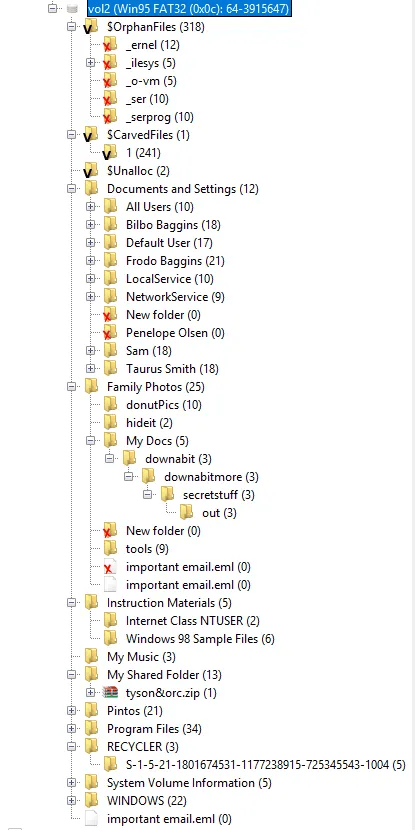
\includegraphics[width=0.6\textwidth]{images/Evidence Examination/Image3.png}
    \caption{Directory Explorer View showing folder structure and suspicious directories}
    \label{fig:directory_explorer}
\end{figure}

As visible in Figure 6.3, the directory structure contains multiple user profiles including "Bilbo Baggins," "Frodo Baggins," "Sam," "Penelope Olsen," and "Taurus Smith." This pattern of multiple user accounts with literary-themed names (from J.R.R. Tolkien's "The Lord of the Rings") suggests deliberate account creation for specific purposes rather than legitimate multi-user functionality. The number in parentheses next to each directory name indicates the file count within that directory.

Of particular interest in the Taurus Smith directory are several suspicious subdirectories:

\begin{itemize}
    \item "Family Photos" (25) - A potentially misleading directory name that may contain sensitive information disguised as personal content
    \item "donutPics" (10) - Explicitly named directory with direct relevance to the alleged recipe theft
    \item "hideit" (2) - Suspiciously named directory overtly suggesting concealment
    \item "My Docs" (5) - Contains nested subdirectories including "downabitmmore" and "secretstuff"
    \item "tools" (9) - Potentially containing software used for steganography or encryption purposes
\end{itemize}

Several "important email.eml" files appear at multiple locations within the directory structure, suggesting deliberate distribution or duplication of communication evidence. The existence of multiple "New folder" directories with zero files also raises suspicion of potential placeholder directories.

Table \ref{table:directory-analysis} outlines the key directories identified during the examination and their forensic significance:

\begin{table}[htbp]
\centering
\begin{tabular}{|p{3cm}|p{9cm}|p{4.5cm}|}
\hline
\textbf{Directory Name} & \textbf{Forensic Significance} & \textbf{Full Path} \\
\hline
All Users & Shared application data repository; potential evidence of installed steganography or encryption utilities & /Documents and Settings/All Users \\
\hline
Application Data & Contains application configuration files and user-specific settings; often overlooked in basic examinations & /Documents and Settings/[User]/Application Data \\
\hline
Desktop & High-access area frequently containing working files or shortcuts to sensitive locations & /Documents and Settings/[User]/Desktop \\
\hline
My Documents & Primary user document storage; standard location for personal and professional files & /Documents and Settings/[User]/My Documents \\
\hline
donutPics & Explicitly relevant directory given investigation context; potential repository for recipe images & /Documents and Settings/Taurus Smith/donutPics \\
\hline
hideit & Explicitly suspicious nomenclature suggesting deliberate information concealment & /Documents and Settings/Taurus Smith/hideit \\
\hline
tools & Potential repository for third-party applications used in data hiding or encryption & /Documents and Settings/Taurus Smith/tools \\
\hline
Family Photos & Possible misdirection through innocuous naming; common technique for sensitive data concealment & /Documents and Settings/Taurus Smith/Family Photos \\
\hline
important email.eml & Direct evidence of communication potentially relevant to corporate espionage & /Documents and Settings/Taurus Smith/important email.eml \\
\hline
Recycler & Standard Windows location for deleted files; may contain partially recoverable evidence & /Recycler \\
\hline
\end{tabular}
\caption{Directory Structure Analysis and Forensic Relevance}
\label{table:directory-analysis}
\end{table}

\section{Unallocated Space Recovery and Analysis}
Unallocated disk space often contains critical evidence as it houses data from deleted files that remain physically present on the storage medium until overwritten. These deleted artifacts frequently provide insights into concealment attempts and data the user intended to remove from the system.

\subsection{Deleted Data Recovery Findings}
Through specialized carving techniques applied to unallocated space, two significant digital artifacts were recovered:

\begin{enumerate}
    \item \textbf{First Unallocated Space File:}
    \begin{itemize}
        \item Identifier: Unalloc\_8524\_1003921920\_1979842560
        \item Path: /img\_Taurus Laptop.001/vol\_vol2/\$Unalloc/Unalloc\_8524\_1003921920\_1979842560
        \item Size: 975,764,480 bytes (approximately 930 MB)
        \item MIME classification: application/octet-stream
        \item Initial binary analysis revealed structured data patterns suggestive of document or spreadsheet formatting
        \item No identifiable text content was recovered from this file, indicating it may have been a temporary or intermediate file created during data processing
    \end{itemize}
    
    \item \textbf{Second Unallocated Space File (Recipe Container):}
    \begin{itemize}
        \item Identifier: Unalloc\_8524\_43768320\_1003921408
        \item Path: /img\_Taurus Laptop.001/vol\_vol2/\$Unalloc/Unalloc\_8524\_43768320\_1003921408
        \item Size: 821,198,336 bytes (approximately 783 MB)
        \item MIME classification: application/octet-stream
        \item Hex analysis revealed embedded text containing what appears to be a proprietary recipe
    \end{itemize}
\end{enumerate}

\begin{figure}[h]
    \centering
    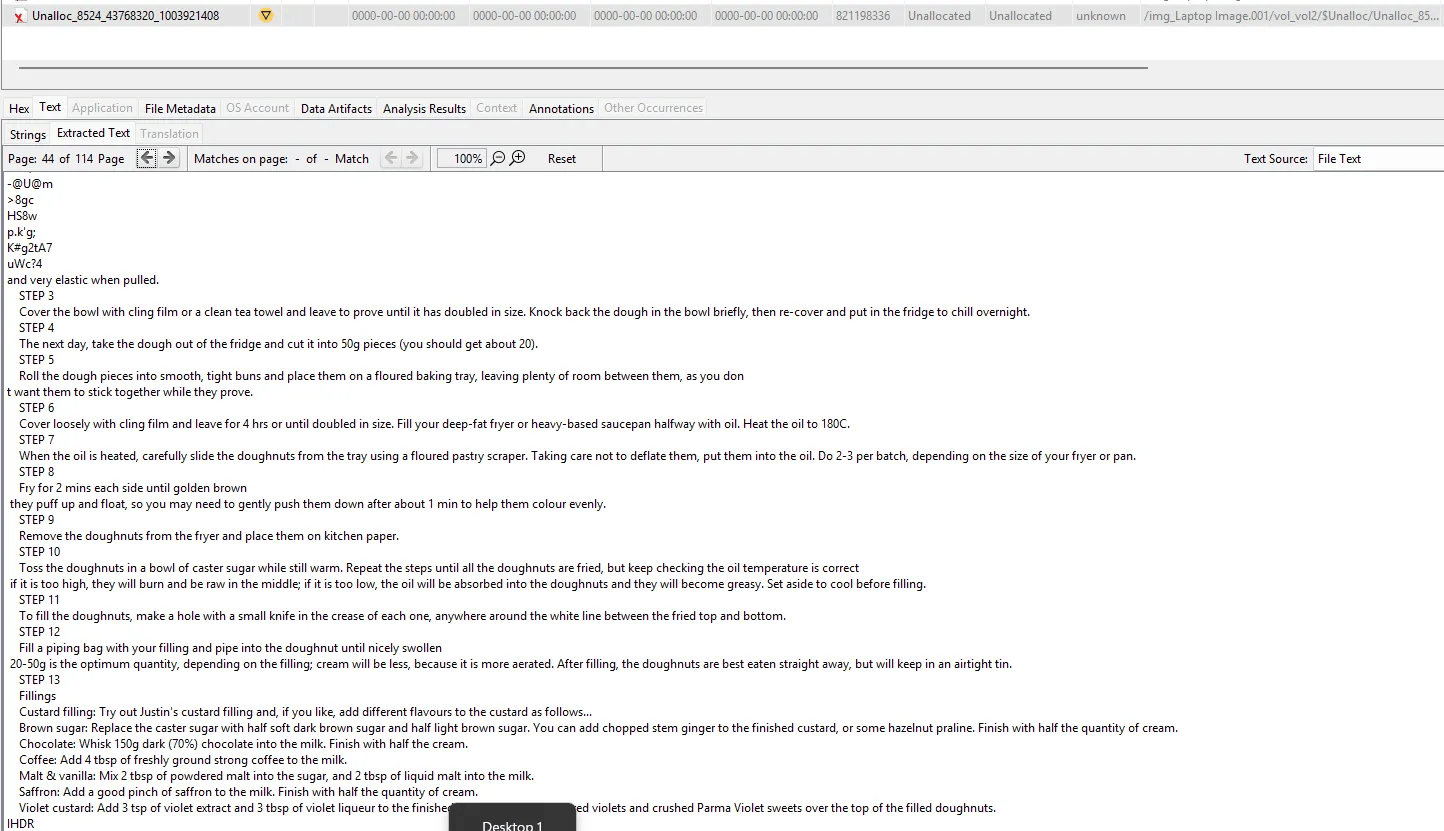
\includegraphics[width=0.95\textwidth]{images/Evidence Examination/Image4.png}
    \caption{Hex View of Recovered Recipe in Unallocated Space showing cooking instructions}
    \label{fig:hex_view}
\end{figure}

\ref{fig:hex_view} shows the text content recovered from the unallocated space, which contains detailed step-by-step instructions for what appears to be a donut recipe. The content includes specific cooking temperatures (180°C for oil), precise measurements (50g pieces of dough), and detailed filling instructions for various flavors including custard, chocolate, coffee, and saffron. The structured format with numbered steps (STEP 3 through STEP 13) indicates this is a formal recipe document rather than casual notes. The technical details about dough consistency, proofing techniques, and cooking methodology suggest this is a professional culinary formula rather than a home recipe.

\subsection{Carving Results and Travel Evidence}
Analysis of carved files from unallocated space yielded additional evidence of significant investigative value:

\begin{figure}[h]
    \centering
    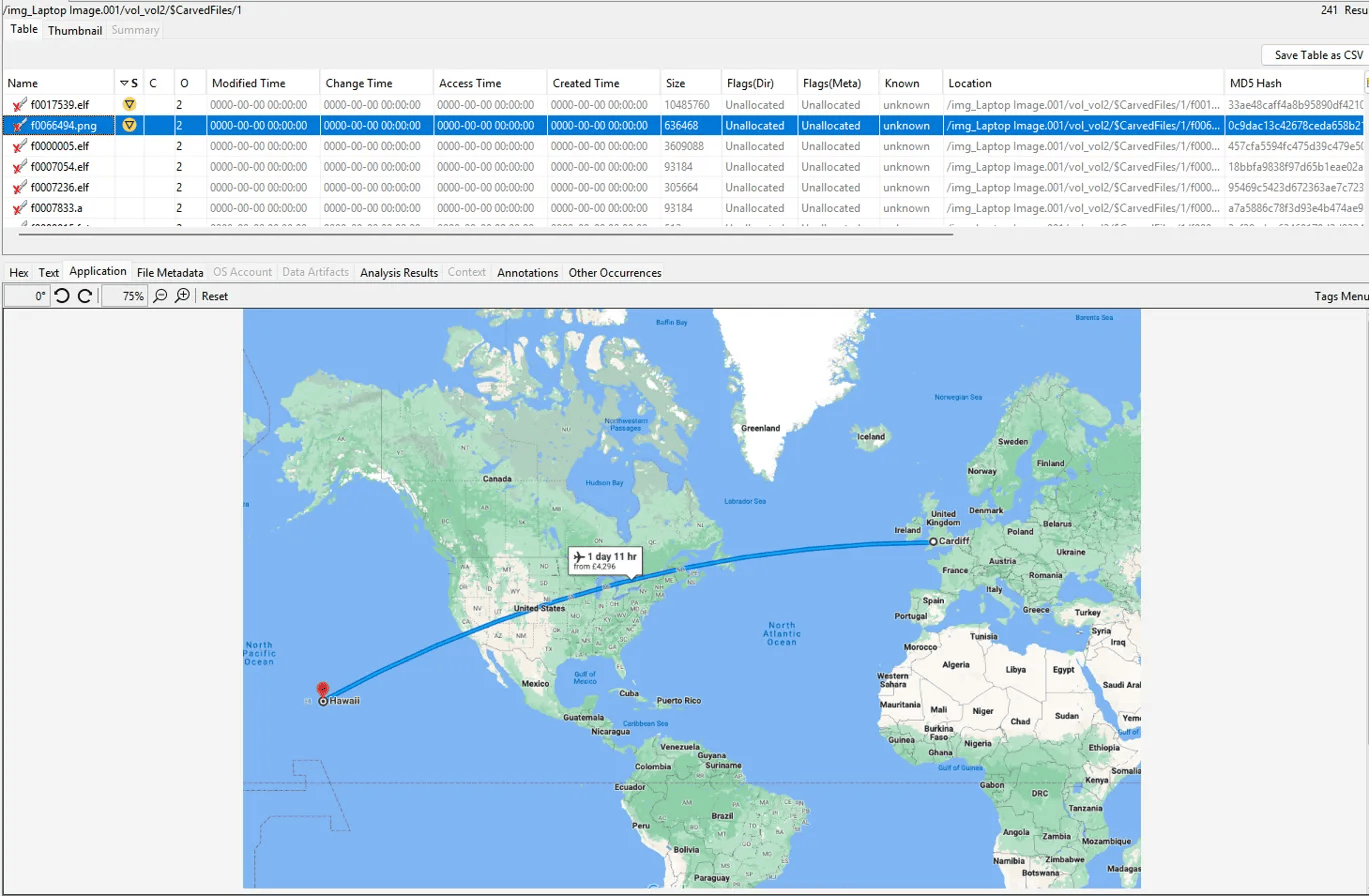
\includegraphics[width=0.95\textwidth]{images/Evidence Examination/Image5.png}
    \caption{Recovered Flight Plan from Cardiff to Hawaii showing travel route and duration}
    \label{fig:flight_plan}
\end{figure}

As shown in Figure \ref{fig:flight_plan}, file f0066494.png was recovered from carved files and contains a map depicting a flight route from Cardiff, Wales to Hawaii. The image shows a travel time of "1 day 11 hr" and appears to be a flight planning document. This evidence directly supports the hypothesis that Taurus Smith was planning international travel, potentially as part of an effort to distribute the proprietary recipe information or meet with collaborators.

The file metadata visible in the table section of Figure 6.5 shows this file is 636,468 bytes in size with "Unallocated" status for both the file name and metadata, indicating it was deleted prior to the image acquisition. The timestamp fields all show null values (0000-00-00 00:00:00), which is consistent with data recovered from unallocated space where filesystem metadata is not preserved.

\subsection{Email Evidence Analysis}
Examination of recovered email artifacts yielded critical evidence directly linking to steganography techniques used to conceal recipe information:

\begin{figure}[h]
    \centering
    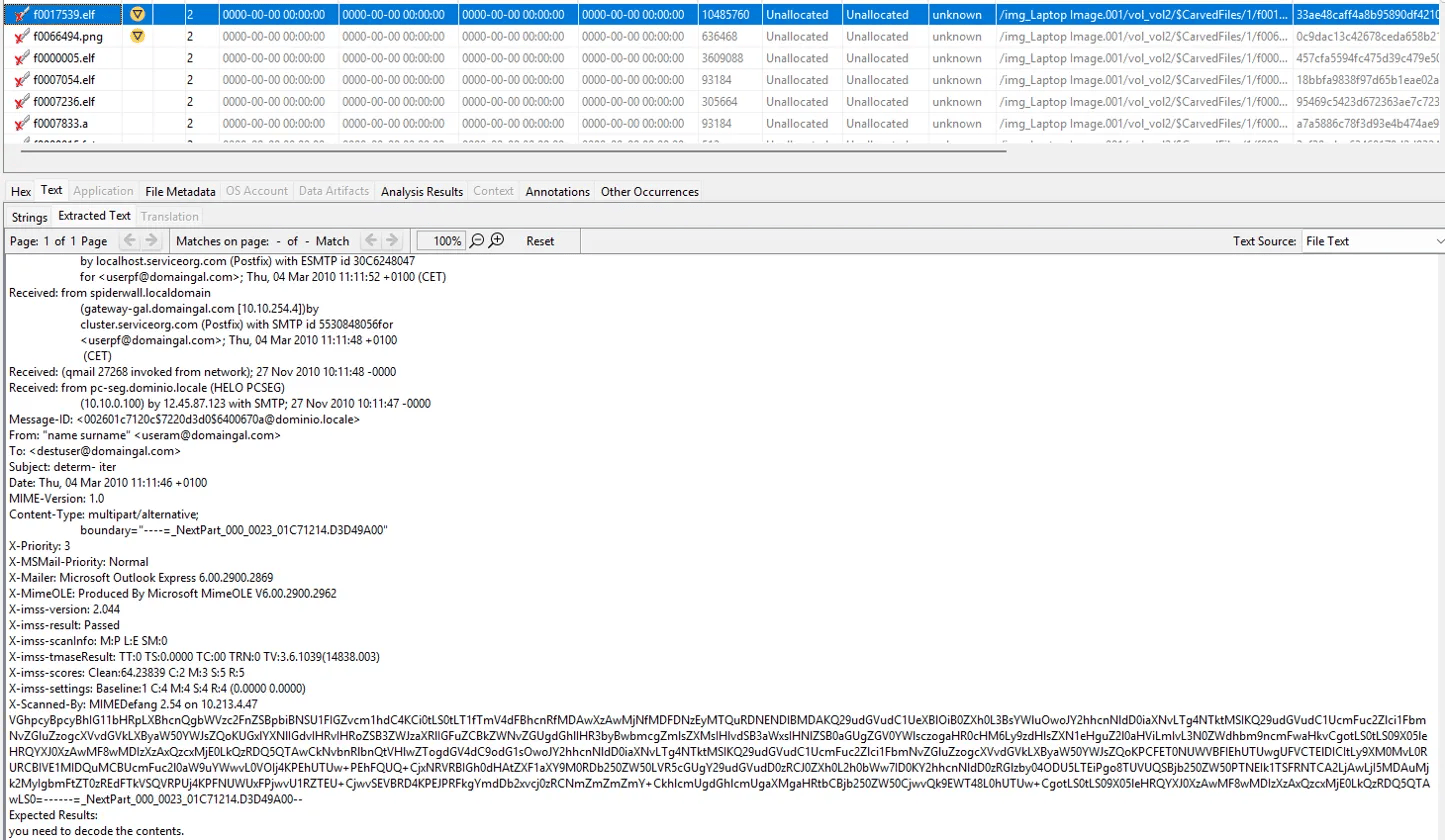
\includegraphics[width=0.95\textwidth]{images/Evidence Examination/Image6.png}
    \caption{Email Artifact Recovery showing Base64-encoded content}
    \label{fig:email_artifact}
\end{figure}

Figure \ref{fig:email_artifact} displays an email artifact recovered from the f0017539.elf file. Initial analysis revealed that the file contained Base64-encoded content. When decoded, this content revealed a multi-part MIME message with both plaintext and HTML components. The plaintext component contained explicit instructions to "go to the website and decode the two png files" with a direct reference to the steganography tool at "https://stylesuxx.github.io/steganography/".

This evidence is particularly significant as it:

\begin{itemize}
    \item Establishes direct knowledge and intent to use steganographic techniques
    \item Specifically references "two png files" that require decoding, likely corresponding (to bean.png and coconuts.png found elsewhere on the system)
    \item Provides the exact steganography tool used (accessible via the referenced URL), enabling investigators to use the same tool to extract hidden content
    \item Contains email header information dating to March 4, 2010, establishing a timeline for these activities
\end{itemize}

The email headers show communication occurring between addresses with the domain "domaingal.com" and contain routing information through multiple servers. The use of Base64 encoding within an .elf file format suggests an additional layer of obfuscation beyond the steganography itself—a technique that would require technical knowledge beyond casual computer use.

This discovery creates a direct investigative link to other image files recovered from the system, particularly those with the .png extension, as they may contain hidden recipe data accessible through the specifically mentioned steganography tool. The deliberate nature of these instructions, combined with the technical steps taken to conceal them, strongly suggests premeditated action rather than incidental activity.
\subsection{Metadata Analysis of Recovered Content}
Detailed examination of the second unallocated file containing recipe information yielded the following metadata characteristics:

\begin{table}[htbp]
\centering
\begin{tabular}{|p{4cm}|p{8cm}|}
\hline
\textbf{Metadata Attribute} & \textbf{Value/Observation} \\
\hline
File System Designation & Unallocated Blocks \\
\hline
Binary Classification & application/octet-stream \\
\hline
Storage Volume & 821,198,336 bytes \\
\hline
Filesystem Entry Status & Unallocated \\
\hline
Metadata Entry Status & Unallocated \\
\hline
Timestamp: Modified & 0000-00-00 00:00:00 (null value) \\
\hline
Timestamp: Accessed & 0000-00-00 00:00:00 (null value) \\
\hline
Timestamp: Created & 0000-00-00 00:00:00 (null value) \\
\hline
Timestamp: Changed & 0000-00-00 00:00:00 (null value) \\
\hline
Cryptographic Verification & Not calculated for preservation purposes \\
\hline
Forensic Tracking & Internal ID 8525 \\
\hline
\end{tabular}
\caption{Forensic Metadata for Recovered Recipe File}
\label{table:recovered_file_metadata}
\end{table}

The absence of valid timestamps (all showing null values) is consistent with data recovered from unallocated space, as filesystem metadata is typically not preserved when files are deleted. The significant size of the file suggests it may have been part of a larger document or dataset before deletion. The classification as application/octet-stream indicates a generic binary format, which is expected when recovering fragmented data where original file headers may be incomplete or missing.

\section{Operating System Environment Analysis}
The operating system configuration provides essential context for understanding the user's digital environment, application usage patterns, and technical capabilities. This analysis helps establish the technological framework within which any alleged criminal activities would have occurred.

\subsection{System Configuration Assessment}
Examination of system artifacts revealed the following configuration details:

\begin{table}[htbp]
\centering
\begin{tabular}{|p{5cm}|p{8.5cm}|}
\hline
\textbf{System Parameter} & \textbf{Configuration Value} \\
\hline
Operating System & Microsoft Windows XP Service Pack 2 \\
\hline
System Architecture & x86 (32-bit) \\
\hline
Product Identifier & 55274-337-8535232-22871 \\
\hline
Windows Installation Path & D:\textbackslash{}WINDOWS \\
\hline
Temporary Files Location & \%SystemRoot\%\textbackslash{}TEMP \\
\hline
System Owner Designation & ADXP \\
\hline
Computer Name & FRODO1 \\
\hline
System Artifact Identifier & -9223372036854775334 \\
\hline
\end{tabular}
\caption{System Configuration Parameters}
\label{table:system_config}
\end{table}

\subsection{System Environment Forensic Implications}
Several notable aspects of the system configuration have direct investigative relevance:

\begin{itemize}
    \item \textbf{Windows XP Service Pack 2:} This operating system, released in 2004 and succeeded by multiple versions, indicates either a legacy system or deliberate use of older technology. Windows XP lacks many modern security features and has well-documented vulnerabilities that could facilitate certain data extraction or concealment techniques.
    
    \item \textbf{Computer Name "FRODO1":} The system hostname references a character from J.R.R. Tolkien's "The Lord of the Rings," which correlates with user account naming patterns observed elsewhere in the evidence (Bilbo Baggins, Frodo Baggins, Sam). This thematic consistency suggests deliberate persona creation rather than arbitrary naming.
    
    \item \textbf{System Owner "ADXP":} This designation differs from the primary user identity (Taurus Smith), indicating either shared system usage or deliberate ownership obfuscation. This discrepancy warrants further investigation to determine if multiple individuals had access to the system.
    
    \item \textbf{Non-Standard Windows Path:} The Windows installation on drive D: rather than the standard C: drive suggests either a non-standard system configuration or possible drive re-lettering. This anomaly could indicate deliberate system modification or the use of additional storage devices.
\end{itemize}

The 32-bit x86 architecture, while standard for Windows XP systems, could impact the types of applications and encryption technologies available to the user. This technical constraint helps establish the scope of potential tools that could have been employed in any alleged corporate espionage activities.

The temporary files directory, a standard location for ephemeral data created during application execution, warrants careful examination for residual artifacts from data processing or transmission activities. Applications frequently create temporary copies of files being accessed, potentially leaving traces of sensitive information even after deletion of the original files.

The system configuration analysis establishes a technological baseline for the investigation and reveals several anomalies that align with potential covert activity. The older operating system, non-standard drive configuration, and the divergence between system owner and primary user identity collectively suggest an environment potentially configured for obfuscation rather than typical personal or business use.